%\addcontentsline{toc}{part}{Discussion}
\chapter{Evaluation of the system: Discussion}
\label{discussion}

This chapter covers the discussion of the tests results presented in section \ref{results}.
It follows the same structure than chapters \ref{methods} and \ref{results}. 
First, the computing performance evaluation of both the nodes and the topics is discussed in section \ref{discussion_computing}. 
Afterwards, the results obtained in the accuracy experiment are explained and justified in section \ref{discussion_accuracy}. 
Chapter \ref{conclusions} is devoted to the improvement of the system based on the observations performed on the experiments. 

\section{Computing performance evaluation}
\label{discussion_computing}
In this section the results obtained when evaluating the computing performance of the system are discussed. 
First, the nodes' CPU and RAM usage is evaluated and afterwards the topic network usage, making a separate reference to the publishing rate and the bandwidth measurements. 

	\subsection{Nodes' CPU and RAM usage}

			The total CPU usage of the system is of a 25\%, which is roughly a single core of the CPU, and the RAM utilization of less than 1 GB of memory. 
			This information suggests that the software is able to run on real time with the hardware used in the experiments. 
			The percentage of the CPU and RAM usage (23\% and 5\% respectively) show that the system would able to work on real time in a computer with lower RAM and slower or smaller CPU than the one used. 
			That is, the minimum requirements for a computer to be able to run this system on real time would be to have at least 1GB of RAM memory and a 1 core processor with a minimum speed of 2,40 GHz or equivalent processing unit.  


		\subsection{Topic network usage}

			Chapter \ref{results} presented the results of the topic network usage experiment. 
			Two different characteristics were measured: the publishing rate and the bandwidth used. 
			That data can be found in the figures \ref{hz} and \ref{bw} respectively. 
			\\

			\begin{itemize}
				\item{\textbf{Publishing rate}}\\

				The bottle neck of the publishing rate of all the nodes is the kinect. 
				Since this sensor is the one that provides the input information to the system, the maximum publishing rate of its nodes will be the one of the kinect, 30 messages per second.
				This figure is high enough to allow the system to perform on real time. 
				In fact, the publishing rate of the output of the system was lowered up to approximately one result per second.
				This reduction of the publishing rate was performed to filter the instantaneous results and hence reduce the noise of the system without damaging its performance.
				Outputting one result per second is fast enough to permit a natural information exchange between the system and its users.
\newpage
			\item{\textbf{Bandwidth}}\\

				The ROS framework allows the distribution of the processing among different devices that are interconnected. 
				The total bandwidth measured in the system is below 7 MB/s, a figure that allows the implementation of this system using a distributed architecture. 
				Nevertheless, the bandwidth of the different network types and technologies must be checked previously to ensure that their bandwidth is high enough. 
				\\

				As an example, a LAN, WAN or MAN network might be introduced to communicate the system since their maximum bandwidth is in the range of the hundreds of megabytes per second. 
				Nevertheless, the communication could not be performed on a Internet network using the 802.11b protocol, whose bandwidth has a maximum of 2 MB/s.
				This does not mean that the system is not able to communicate through the Internet. 
				Other protocols created later such as the 802.11n have a much higher maximum bandwidth, in the range of the hundreds of megabits per second.

			% Si los nodos permiten un cómputo en tiempo real y si la carga del sistema a la red permite que se pueda distribuir (al menos sobre el papel)  los nodos de tu sistema entre varias máquinas. 


		\end{itemize}

\section{Evaluation of the object recognition accuracy}
\label{discussion_accuracy}
	This section discusses the results obtained in the accuracy measurement experiment. 
	To consult them please refer to section \ref{results_accuracy_measurement}.
	Each different experiment is discussed in a different subsection.


	\subsection{Template using 1 view}
	The tables that show the confusion matrix of the experiment and the precision, recall and F1 score obtained are \ref{1view_matrix} and \ref{1view_fscore} respectively. 
	The results show that the system outputted the skull, cup, bottle and mobile a noticeable amount of times when each of them were being used. 
	This could be due to the similarity in the 2D texture in the skull, cup and bottle and and 3D similarity of the cup, when presented occluding the holder, the bottle and the mobile. 

	\begin{figure}[h]
		\begin{center}
	    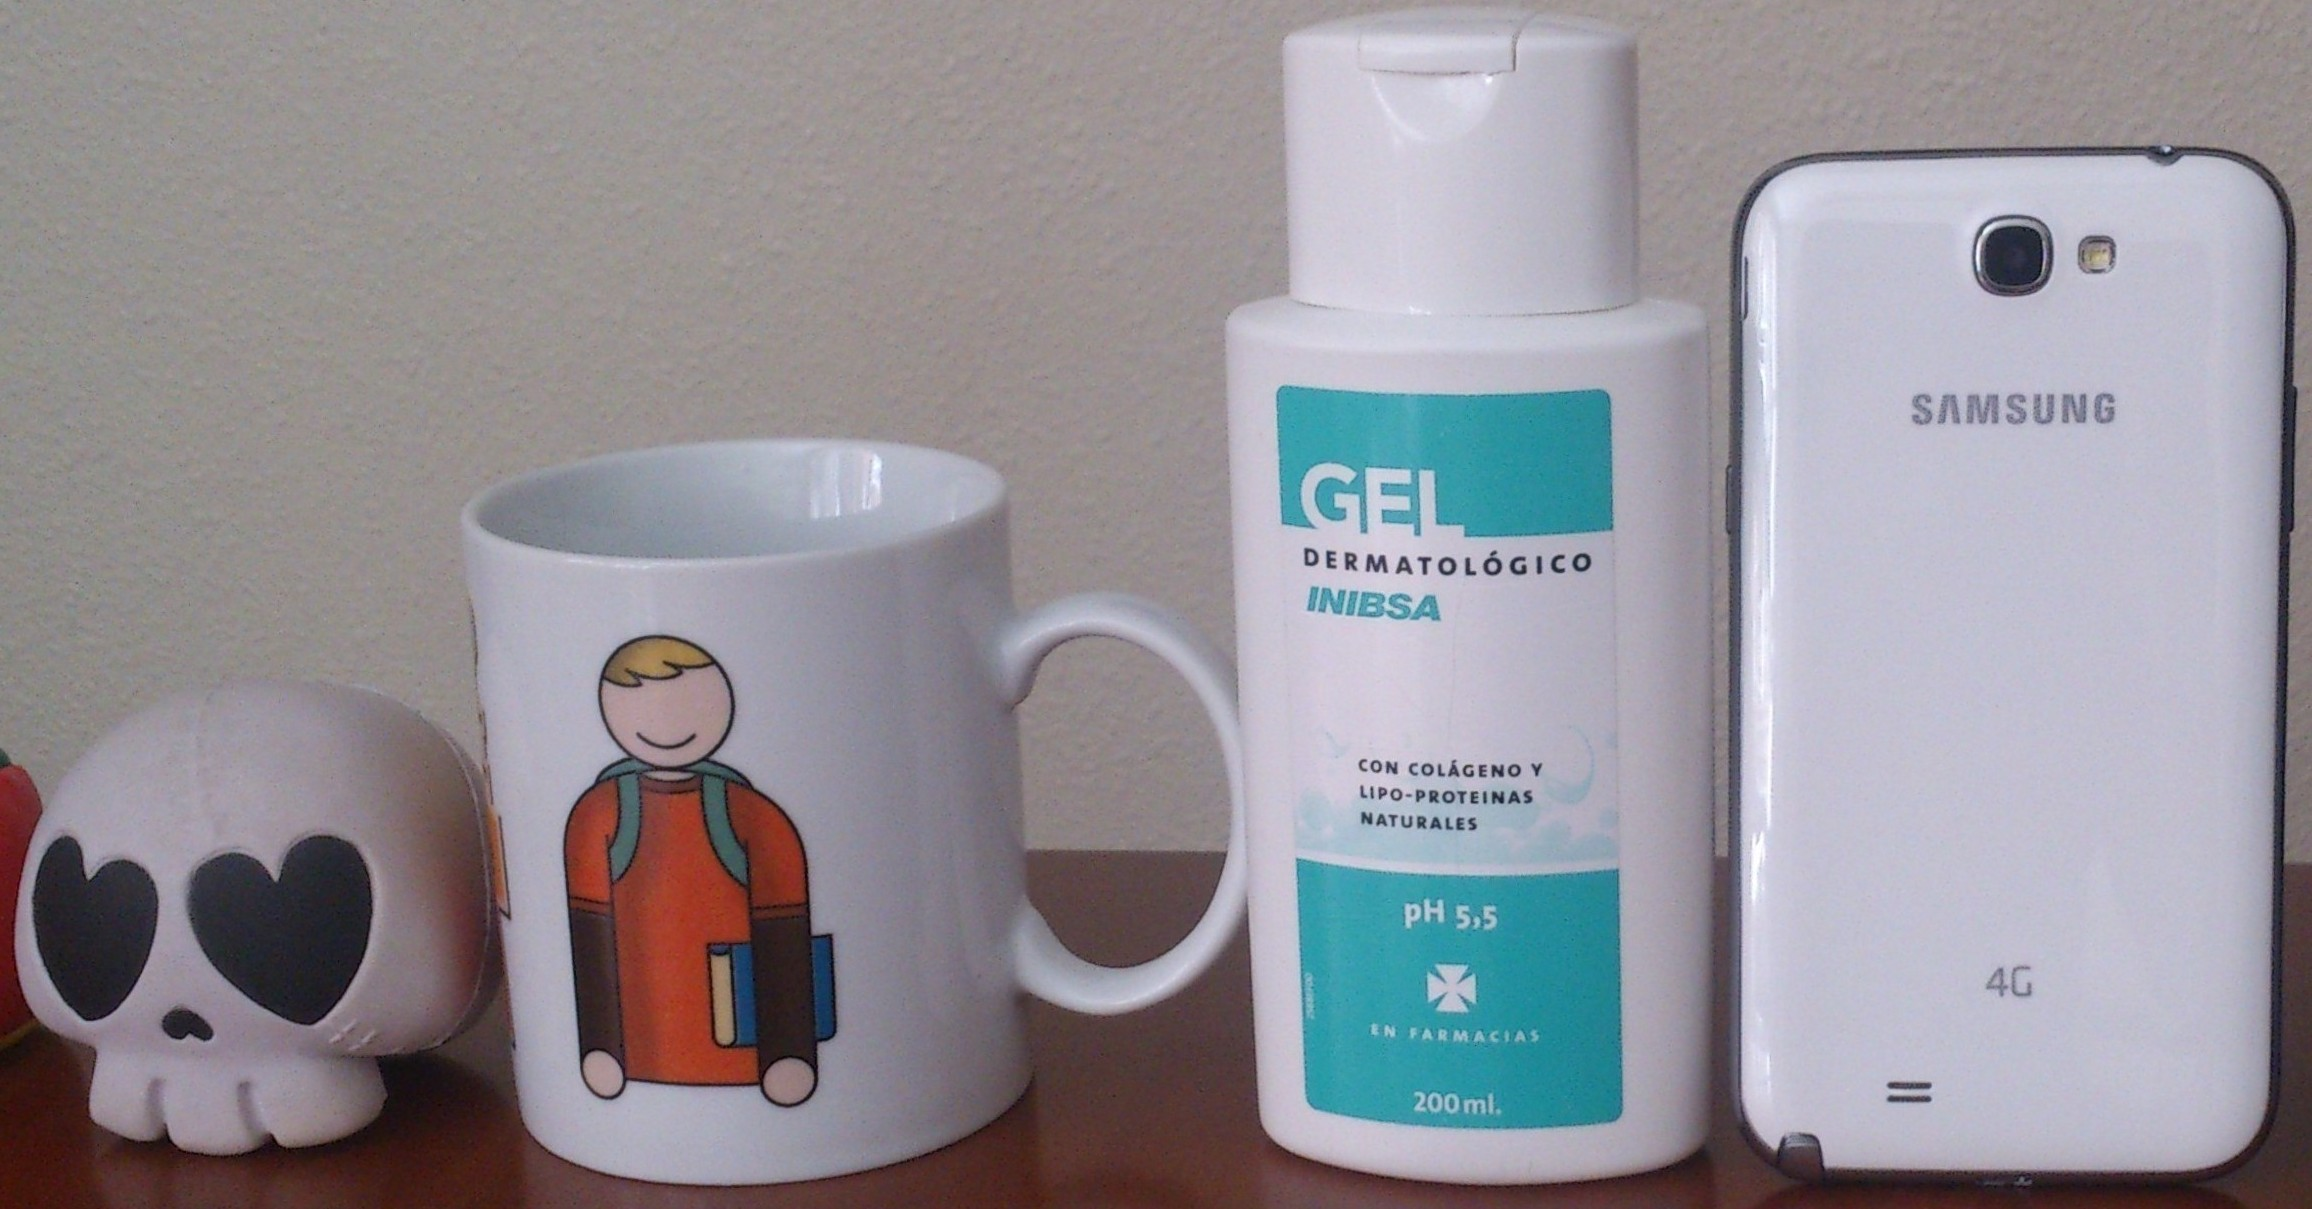
\includegraphics[width=\linewidth]{img/discussion/comparison1.jpg}
		\caption[Comparison: Skull, cup, bottle and mobile]{Detail of the skull, cup, bottle and mobile objects to illustrate their similarities. }
		\label{comparison1}
		\end{center}
	\end{figure}

	As it can be seen in figure \ref{comparison1}, the 2D details of the highly textured cup and bottle and also those of the skull present round lines that could have created similar 2D descriptors. 
	Also, the 3D form of the cup, the bottle and the mobile is very similar which might lead as well to the creation of matchable 3D descriptors in the borders. 
	\\

	The cup's results are similar to the ball's. 
	The precision and recall are similar in number and low. 
	The features extracted from this object were not descriptive enough.
	The most descriptive features were obtained from the calculator, an object that presents an F1 score of 65\% in this experiment. 
	% % It was confused with the mobile and the bottle, probably due to the similarity in 2D texture as was the case with the skull. 
	% Also, the cup was outputted when all the other objects in the dataset were being used, with a specially high ratio in the skull and mobile. 

	%ampliar para el resto de objects!

	\subsection{Template using 5 views}
	\label{discussion_5views}

	The skull obtained approximately a 0.6 success rate, and most of the ball almost 0.4 recognition ratio when the skull was being used in the system. 
	% Most of the 40\% of recognitions were ball. 
	This results supports the theory that the 3D similarity between those objects, which may be seen in figure \ref{comparison2} may lead to very similar 3D descriptors. 

\vspace{0.5cm}
	\begin{figure}[h]
		\begin{center}
	    \includegraphics[width=\linewidth]{img/discussion/comparison2.png}
		\caption[Comparison: ball and skull]{Detail of the ball and the skull using different views to illustrate their 3D similarities. }
		\label{comparison2}
		\end{center}
	\end{figure}


\vspace{0.5cm}
	The skull was recognized a ratio of 0.2 when the cup was being shown to the system, which is a high value. 
	The reason behind it could be the similarity in the 2D texture of skull and cup. 
	Both are white objects with drawings that contrast with that background, as can be seen in figure \ref{comparison1}. 
	\\
	
	Figure \ref{5views_matrix} shows that when the mobile was shown to the system, the skull, the ball and the bottle were detected. 
	The mobile has rounded corners and sides that could make 3D descriptors on those locations be similar to the previous objects. 
	Also, the mobile is white with details represented in the 2D texture. 
	This feature is common with the bottle and the cup. 
	For certain positions of the cup and the mobile the 2D projection could be similar and lead to obtain less representative descriptors of the object. 
	These similarities between the skull and the bottle may be seen in figure \ref{comparison1}.

\newpage

	\subsection{Template using 10 views}
	The results of this experiment may be found in figures \ref{10views_matrix} and \ref{10views_fscore}. 
	It can be observed an improvement with respect to the previous measurements. 
	Now, all success rates and F1 scores of the objects are above the 69\%. 
	Also it can be seen that the number of false recognitions was reduced noticeably mainly in the bottle, mobile and calculator objects. 
	\\

	% Figure \ref{10views_fscore} presents much better results than the previous experiments (Figures \ref{1view_fscore} and \ref{5views_fscore}).
	The bottle is the object with a higher F1 score of the whole experiment. 
	This implies that the augment of the number of learned views improve the accuracy of the system limiting the high amount of false positives obtained in the experiments using 1 and 5 views. 
	It is noticeable that the bad precision presented in the ball recognition limited its F1 score result. 
	This was caused by the outputting of the ball when all the other objects were being used. 
	The ball was detected wrongly a high amount of times when the skull and the calculator were being shown.
	The first case was already explained in section \ref{discussion_5views}: the ball and the skull have very similar 3D form. 
	The second case might be because of the fact that both objects have high 2D texture composed of straight lines and the 2D descriptors extracted might have been very similar. 
	\\

	The results of the experiment using ten views are very promising. 
	Since there is an almost proportional relation between the F1 score and the number of views learned per object, further measurements could be performed to determine the optimum balance between F1 score and processing requirements. 
	
	\subsection{Comparison of the 2D and 3D independent recognition results and the system's output}

	The comparison performed of the F1 score results for the 2D and 3D independent recognition processes and the final system's output, which combines both of them showed that the combination of results improves the F1 score. 
	It is noticeable that the 3D algorithm obtained lower results in all the cases but one than the 2D. 
	This fact corroborates the usefulness and correctness of the decision step performed in the system, in which a higher importance was given to the 2D predictions (see section \ref{last_node}).
	\\

	It is also important to remark that further experiments may be performed to adapt better the importance given to each algorithm in the decision procedure.
	It is possible to even adapt it to the different situations and objects that could appear. 
	Further details are explained in section \ref{future_decision}.